\subsection{Kohlenstoffkreislauf}

\begin{frame}
	\frametitle{Kohlenstoffkreislauf}
	\begin{columns}
		\column{0.25\linewidth}
		\begin{figure}
			\centering
			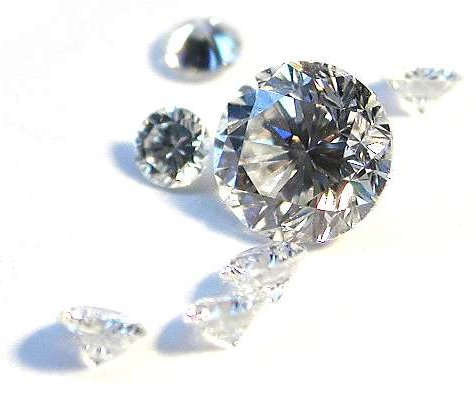
\includegraphics[width=\linewidth]{bilder/kohlenstoff/Brillanten}
			\caption{Diamant, 100\% Kohlenstoff, Bildquelle: Wiki1}
		\end{figure}
		\column{0.25\linewidth}
		\begin{figure}
			\centering
			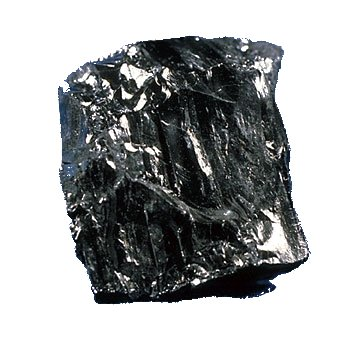
\includegraphics[width=\linewidth]{bilder/kohlenstoff/kohle}
			\caption{Anthrazit Kohle, $\geq\,90$\% Kohlenstoff (trocken), Bildquelle: Wiki2}
		\end{figure}
		\column{0.25\linewidth}
		\begin{figure}
			\centering
			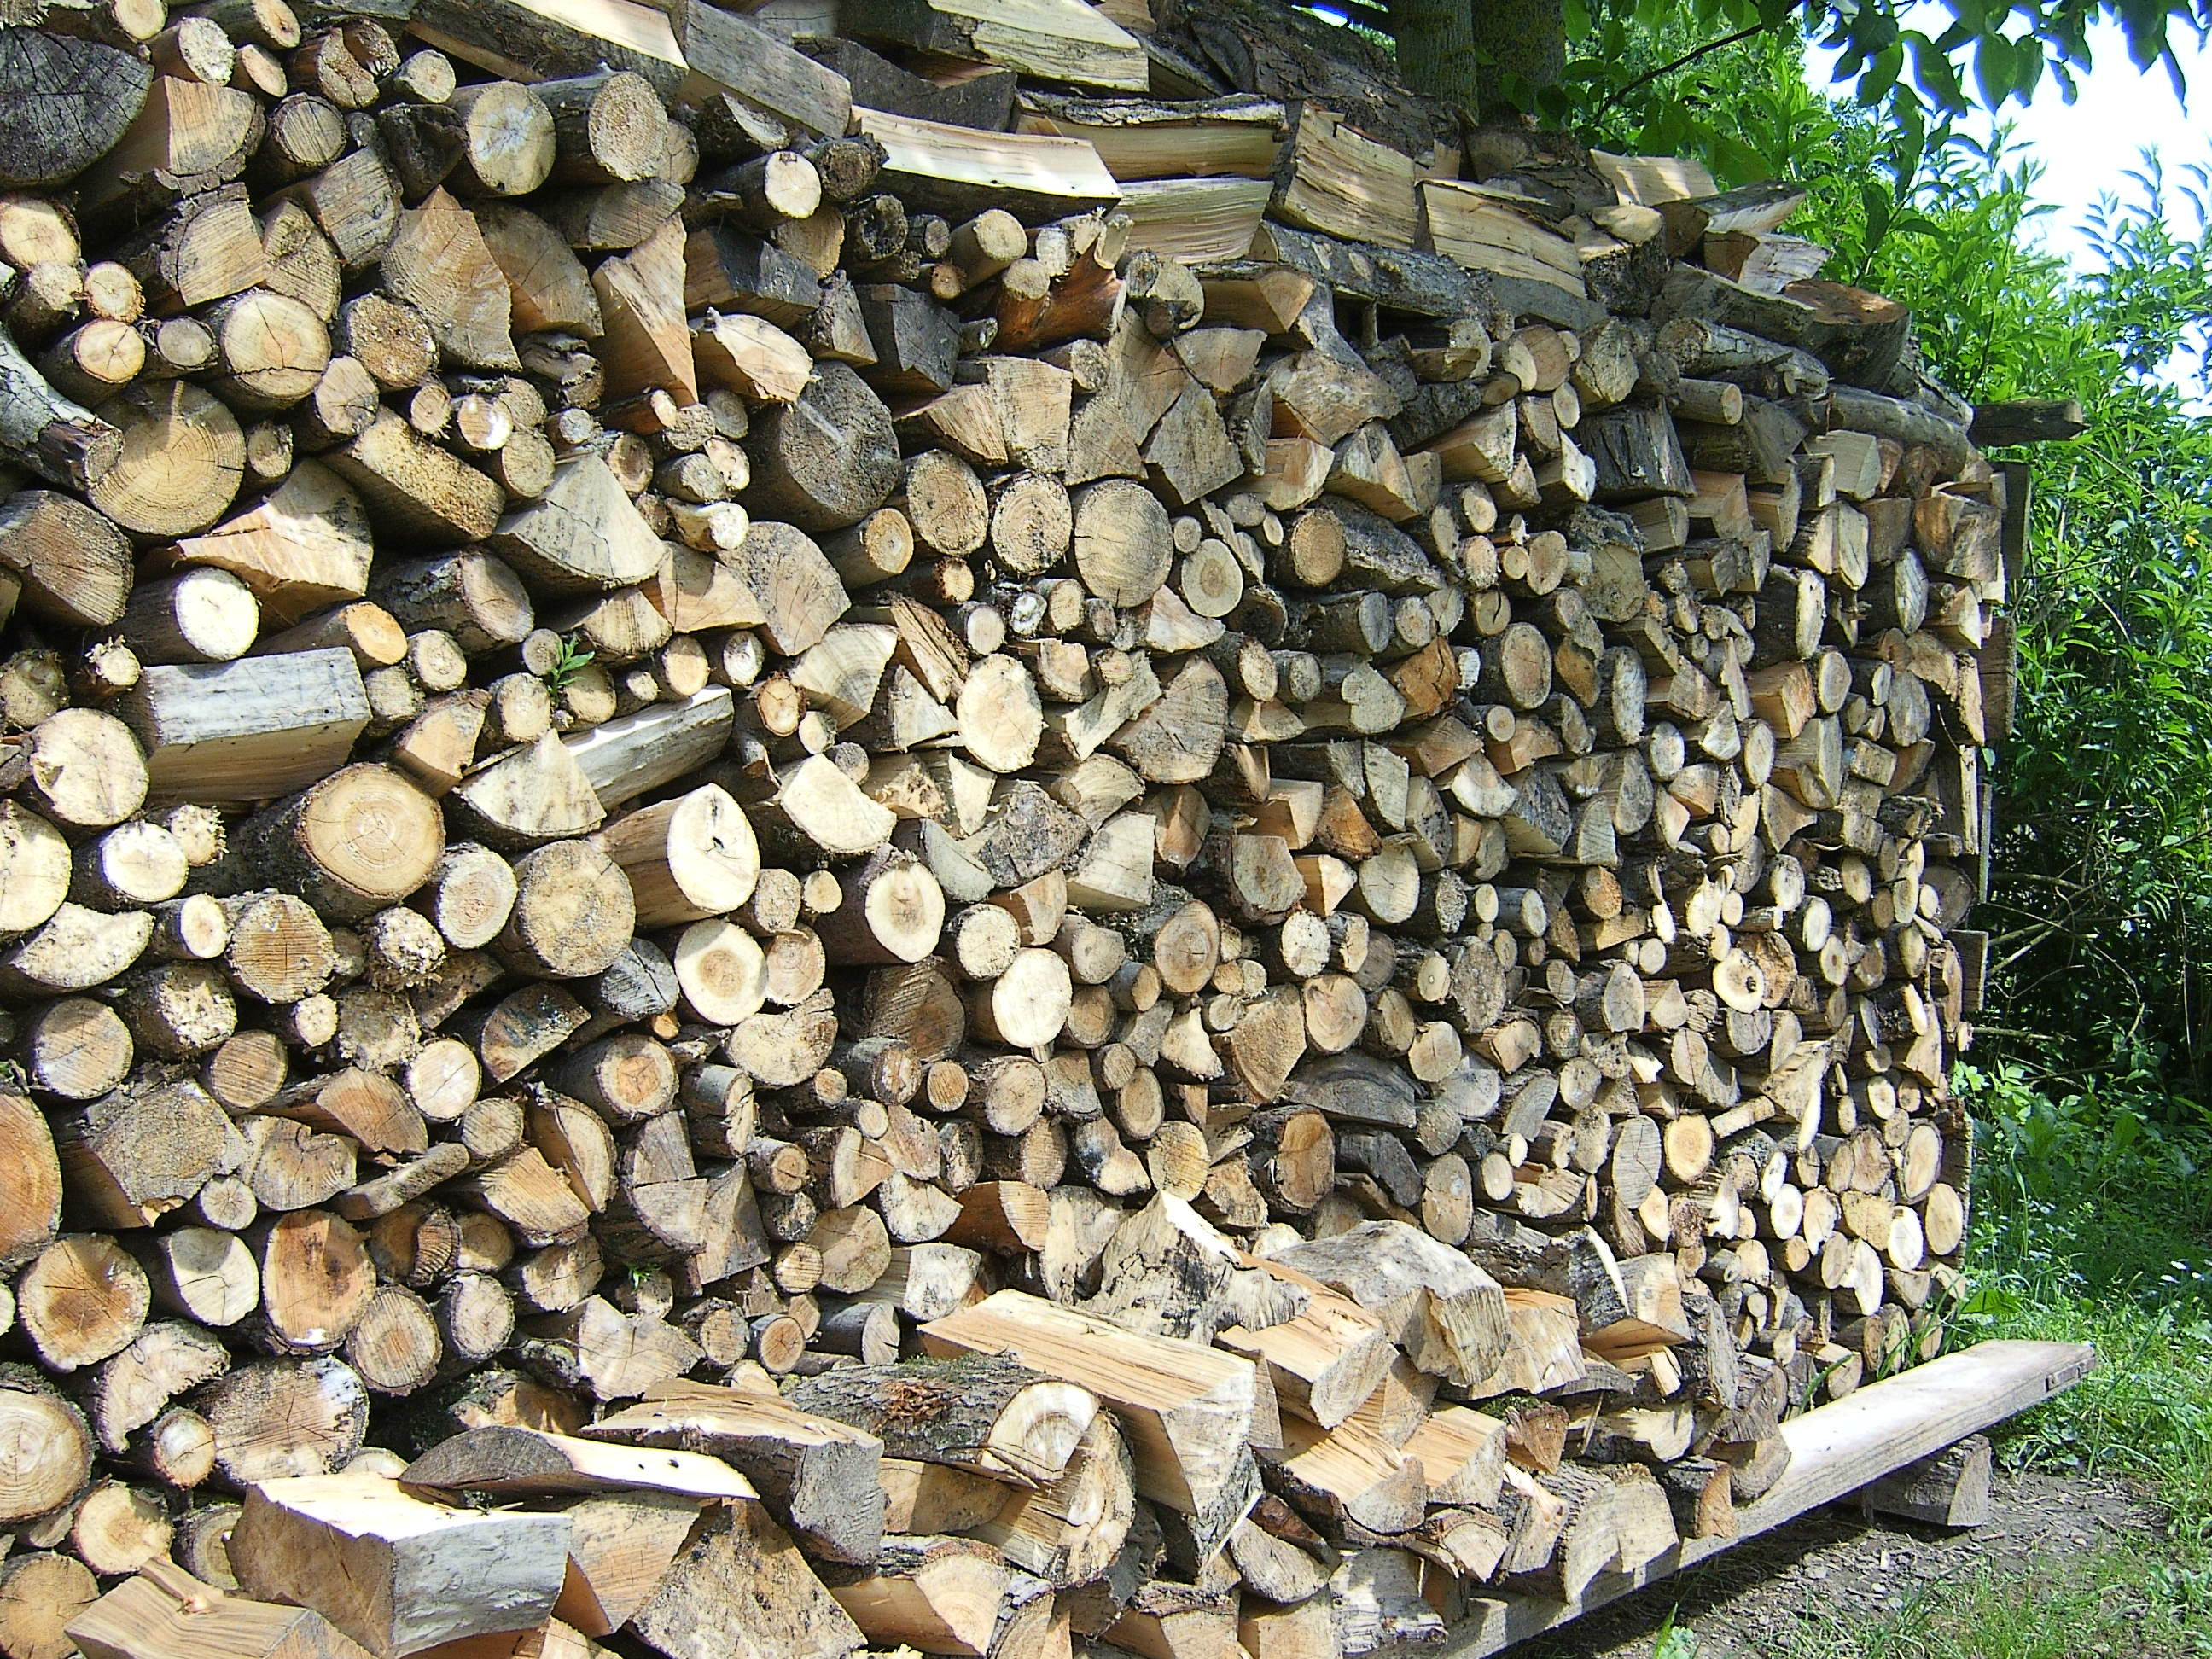
\includegraphics[width=\linewidth]{bilder/kohlenstoff/holz}
			\caption{Holz, $\approx 50$\% Kohlenstoff (trocken), Bildquelle: Wiki3}
		\end{figure}
		\column{0.25\linewidth}
		\begin{figure}
			\centering
			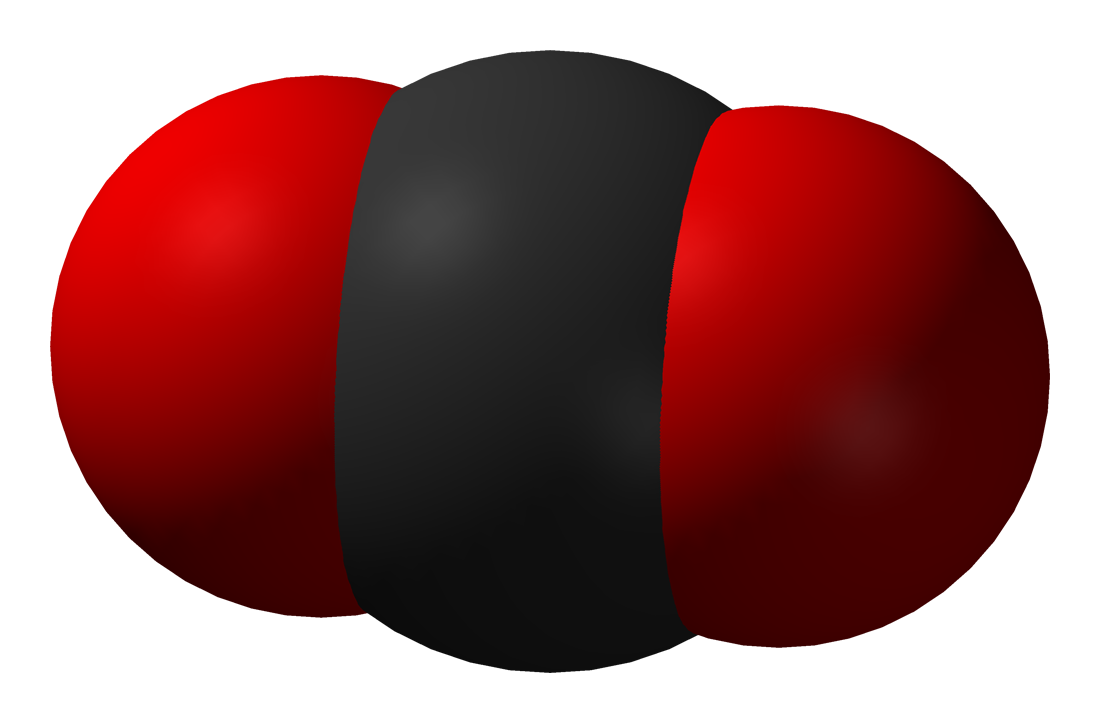
\includegraphics[width=\linewidth]{bilder/kohlenstoff/co2}
			\caption{Kohlenstoffdioxid $\text{CO}_2$, Ein Kohlenstoff und zwei Sauerstoff Atome, Bildquelle: Wiki4}
		\end{figure}
	\end{columns}
		\begin{itemize}
			\item Kohlenstoff als reiner Stoff (Diamant, Graphit) oder als Verbindung mit anderen Elementen
			\item Kohlenstoff ist ein Grundbaustein des Lebens
			\item Grundlage der organischen Chemie
			\item Ist Bestandteil von Pflanzen und Tieren
			\item Im Boden gebunden und als Gas in der Atmosphäre
		\end{itemize}

	\note{
		\begin{itemize}
			\item[] Was ist das chemische Element Kohlenstoff überhaupt?
			\item[] Angaben in Massenanteilen
			\item[] Kohlenstoff ist das 11. häufigste Element auf der Erde ({\color{green}Nichtmetall}, {\color{brown}Halbmetall},
			{\color{orange}Erdalkalimetall}, {\color{orange!50!red}Alkalimetall},
			{\color{gray}Metall}, Übergangsmetall)
			\begin{itemize}
				\item[1-3] {\color{green}Sauerstoff}, Eisen, {\color{brown}Silicium},
				\item[4-6] {\color{orange}Magnesium}, Nickel, {\color{orange}Calcium},
				\item[7-9] {\color{gray}Aluminium}, {\color{green}Schwefel}, Chrom,
				\item[10-12] {\color{orange!50!red}Natrium}, {\color{green}Kohlenstoff}, Mangan
			\end{itemize}
		\end{itemize}
	}
\end{frame}

\begin{frame}
	\frametitle{Kohlenstoffkreislauf}
	\begin{columns}
		\column{0.6\linewidth}
		\begin{figure}
			\centering
			\only<1|handout:0>{
				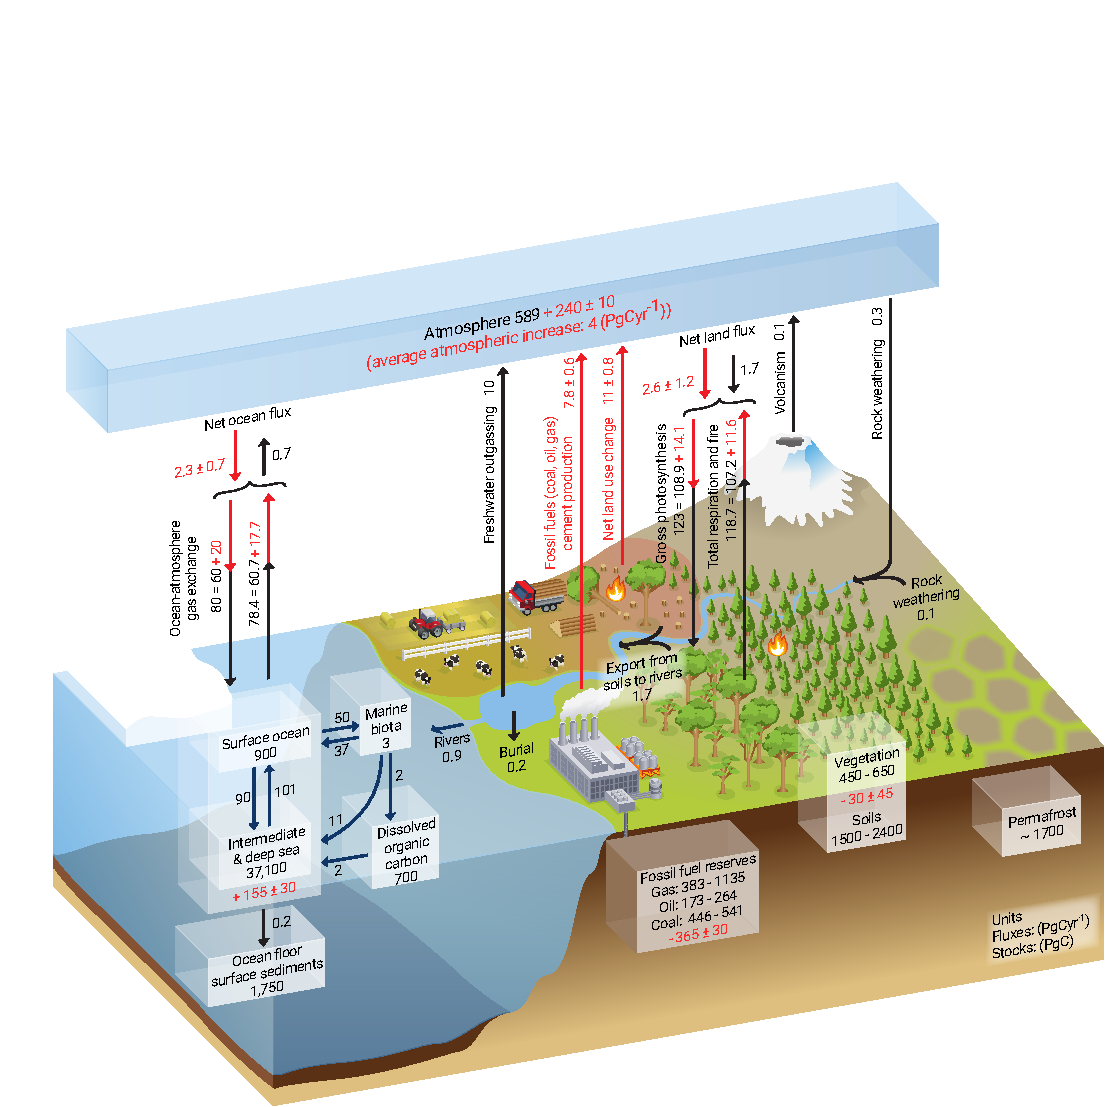
\includegraphics[trim={1cm 0cm 0cm 3cm}, clip, width=0.9\linewidth]{bilder/kohlenstoff/carbon_cycle_industrial-ocean.pdf}
				\caption{Vereinfachte Abbildung zum jährlichen Kohlenstoffkreislauf, Quelle: IPCC 2013, Kapitel 6}
			}
			\only<2|handout:0>{
				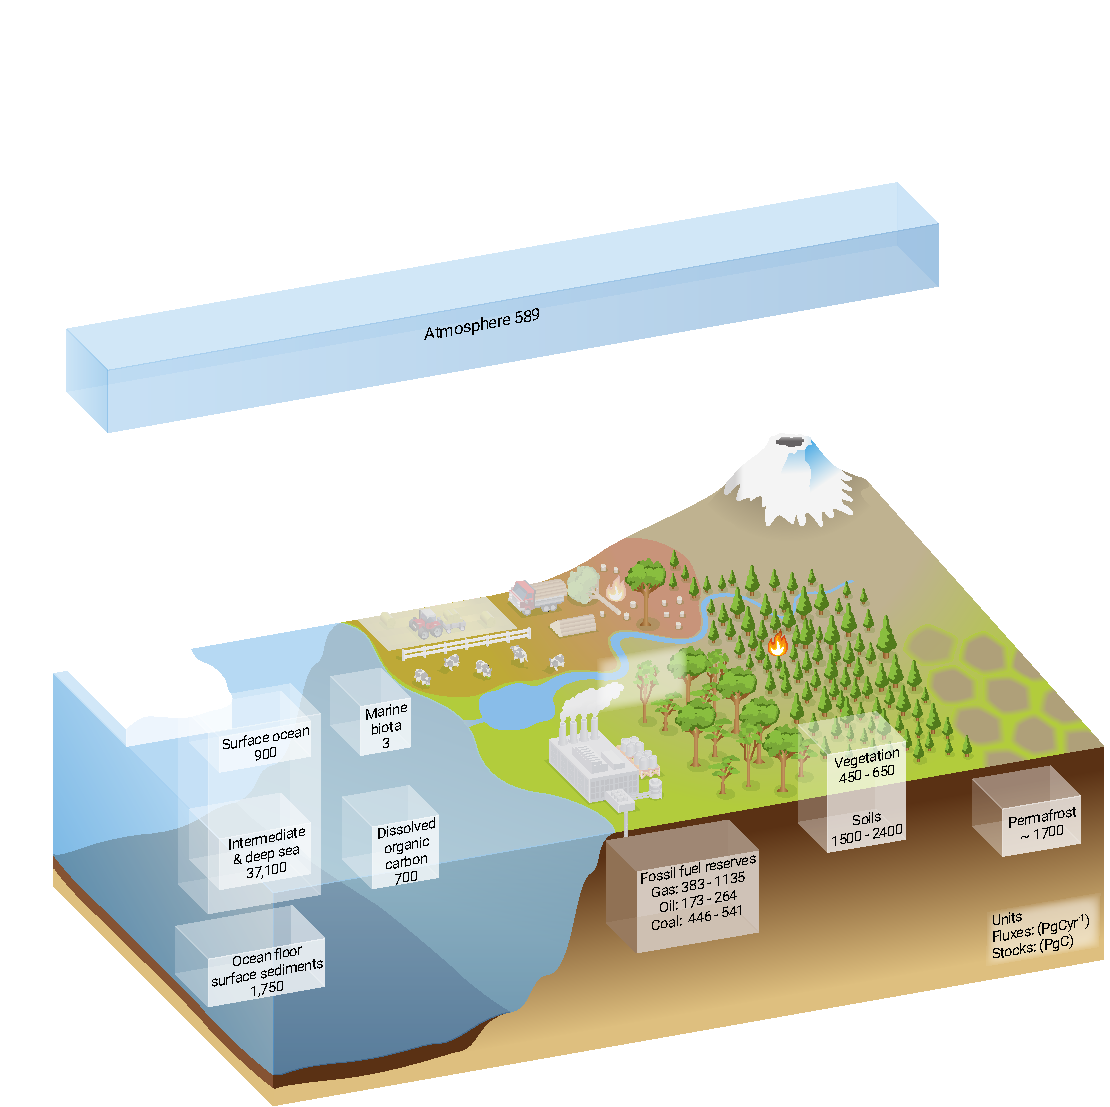
\includegraphics[trim={1cm 0cm 0cm 3cm}, clip, width=0.9\linewidth]{bilder/kohlenstoff/carbon_cycle_reservoirs.pdf}
				\caption{Kohlenstoffspeicher des Erdsystems.}
			}
			\only<3|handout:0>{
				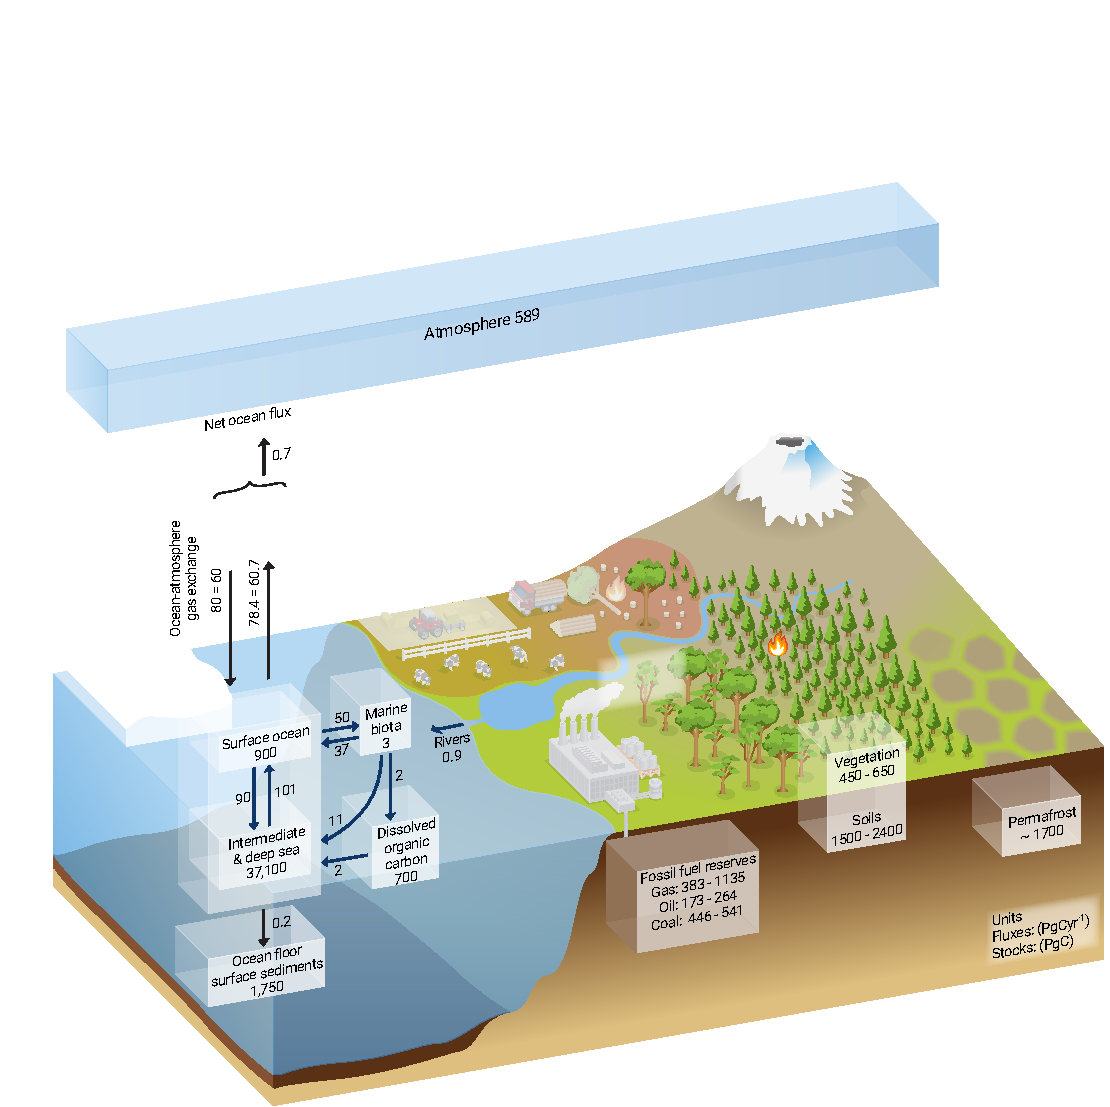
\includegraphics[trim={1cm 0cm 0cm 3cm}, clip, width=0.9\linewidth]{bilder/kohlenstoff/carbon_cycle_ocean-atmosphere.pdf}
				\caption{Wechselwirkungen zwischen Ozeanen und Atmosphäre.}
			}
			\only<4|handout:0>{
				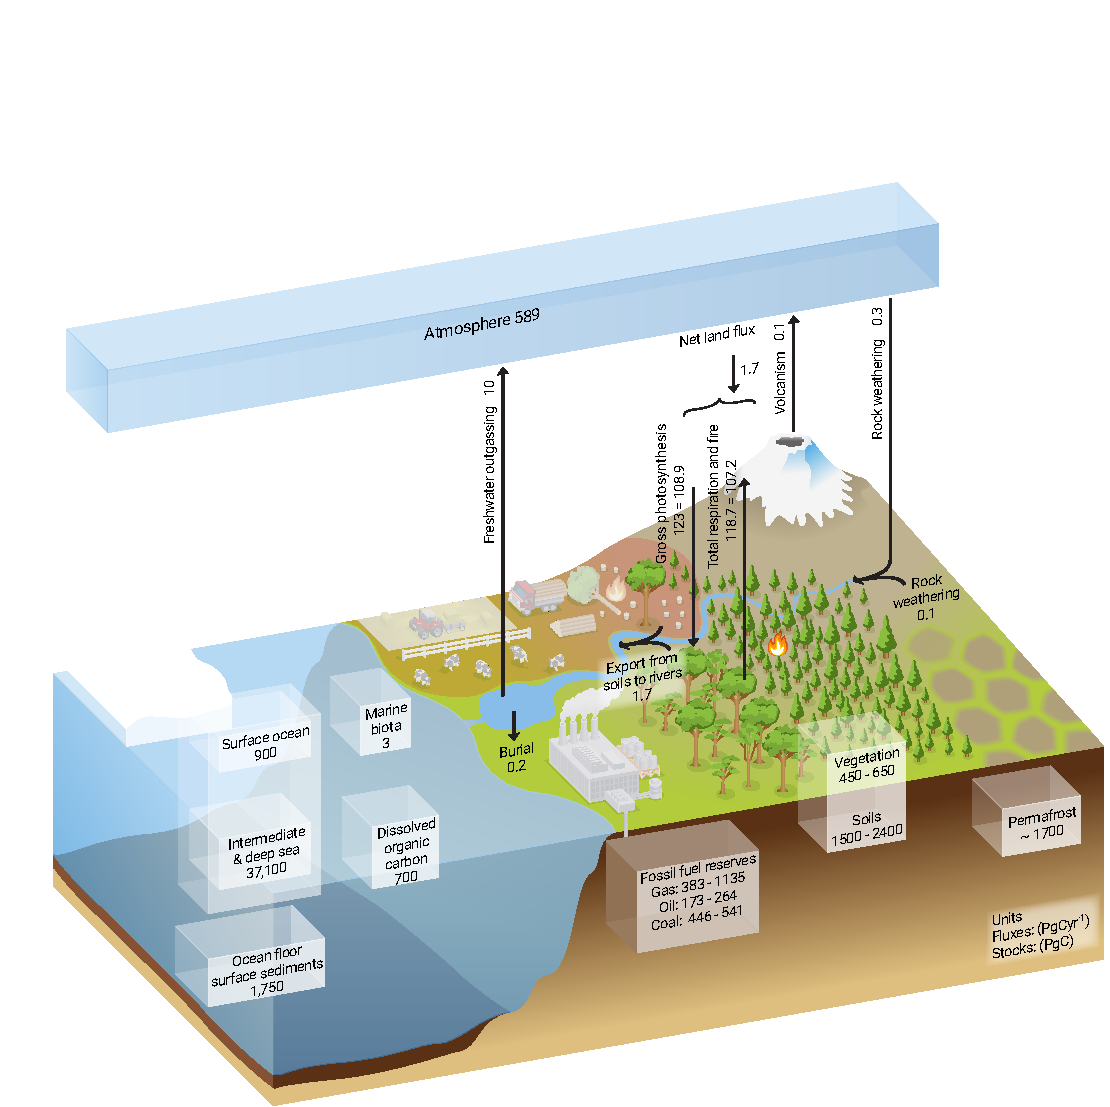
\includegraphics[trim={1cm 0cm 0cm 3cm}, clip, width=0.9\linewidth]{bilder/kohlenstoff/carbon_cycle_pre-industrial.pdf}
				\caption{Wechselwirkungen zwischen Landmassen und Atmosphäre.}
			}
			\only<5|handout:0>{
				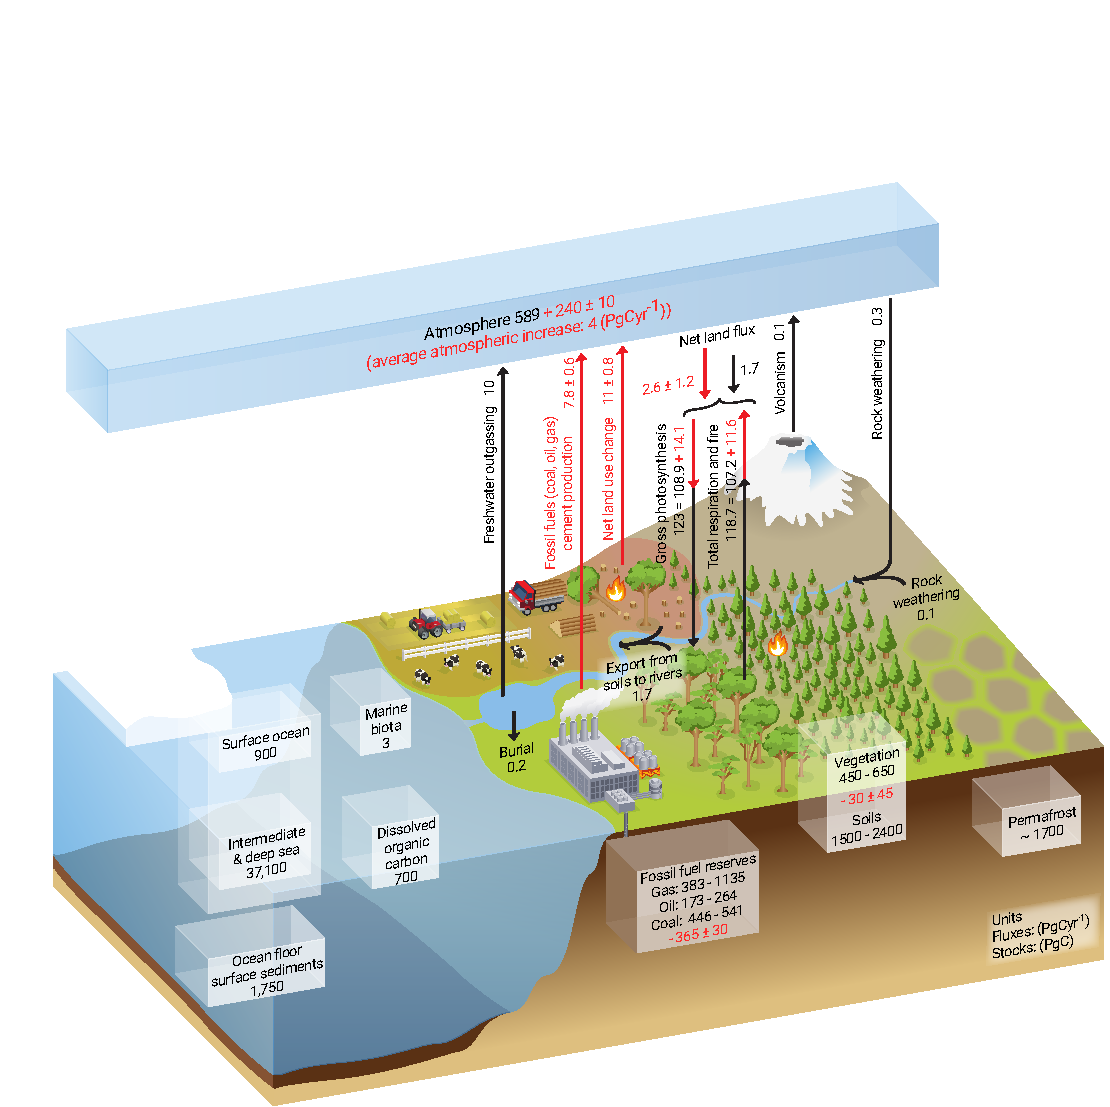
\includegraphics[trim={1cm 0cm 0cm 3cm}, clip, width=0.9\linewidth]{bilder/kohlenstoff/carbon_cycle_industrial.pdf}
				\caption{Anthropogener Einfluss im Kreislauf zwischen Landmassen und Atmosphäre.}
			}
			\only<6|handout:1>{
				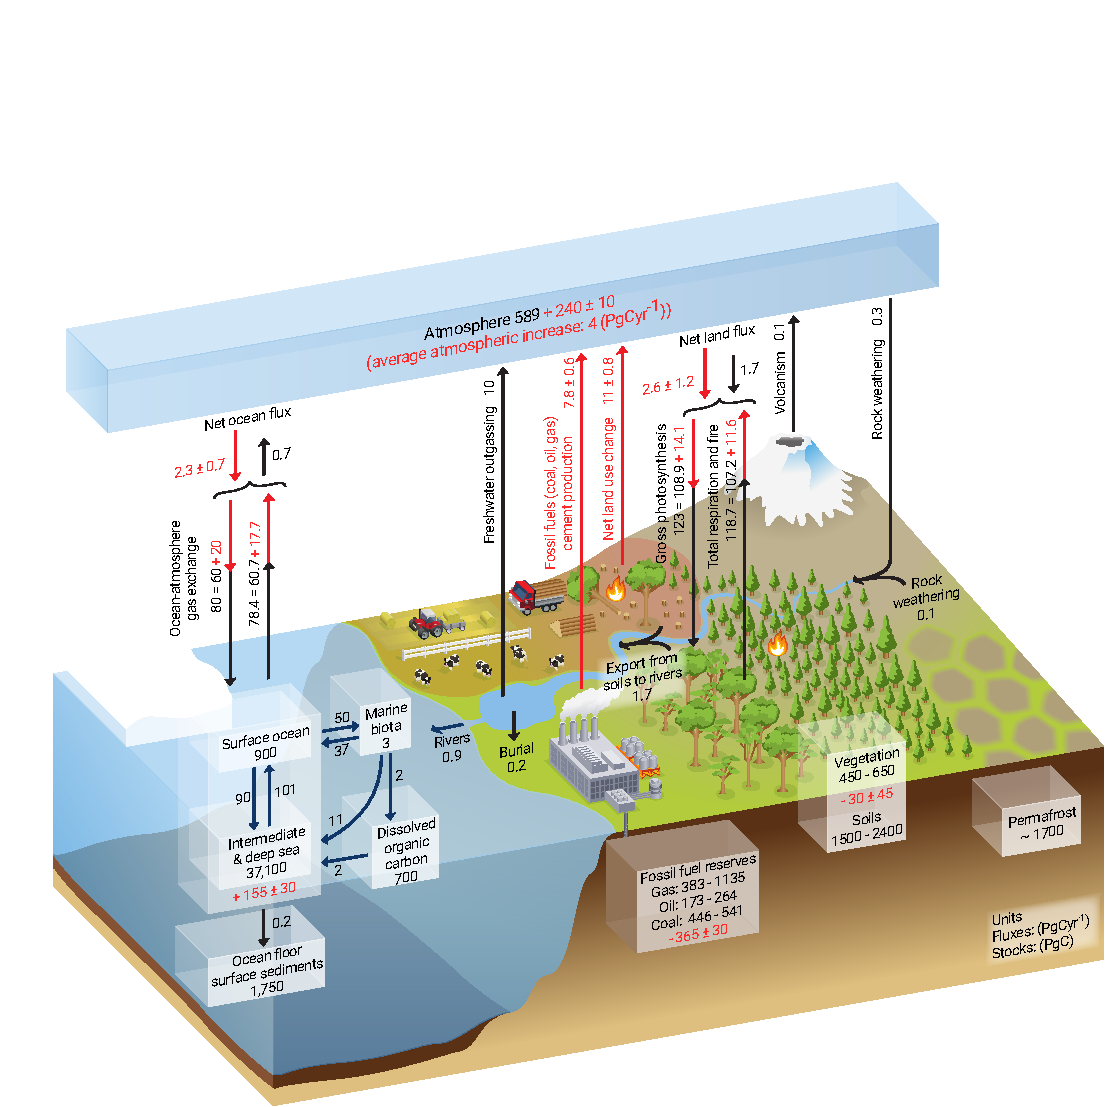
\includegraphics[trim={1cm 0cm 0cm 3cm}, clip, width=0.9\linewidth]{bilder/kohlenstoff/carbon_cycle_industrial-ocean.pdf}
				\caption{Anthropogener Einfluss im gesamten Kohlenstoffkreislauf.}
			}
		\end{figure}
		\column{0.4\linewidth}
		\only<1|handout:0>{
		\begin{itemize}
			\item[\textbf{\rightarrow}] vermutete natürliche CO$_2$-Flüsse vor der Industrialisierung (vor 1750)
			\item[{\color{red}\textbf{\rightarrow}}] durch Menschen verursachte mittlere jährliche CO$_2$-Flüsse (2000 - 2009)
			\item[] \color{red}\textbf{rote Reservoire}\color{black}: kumulative Änderung zwischen 1750 und 2011
		\end{itemize}
		}
		\only<2|handout:0>{
			\begin{itemize}
				\item[] \textbf{Schwarze Zahlen} beschreiben gesamte geschätze Vorkommen in den jeweiligen Reservoiren.
			\end{itemize}
		}
		\only<3|handout:0>{
			\begin{itemize}
				\item[] \textbf{Schwarze \rightarrow} sind geschätzte natürliche CO$_2$-Flüsse vor der Industrialisierung (vor 1750)
			\end{itemize}
		}
		\only<4|handout:0>{
			\begin{itemize}
				\item[] \textbf{Schwarze \rightarrow} sind geschätzte natürliche CO$_2$-Flüsse vor der Industrialisierung (vor 1750)
			\end{itemize}
		}
		\only<5|handout:0>{
			\begin{itemize}
				\item[] \color{red}\textbf{Rote \rightarrow} \color{black} sind durch Menschen verursachte mittlere jährliche CO$_2$-Flüsse von zwischen 2000 und 2009.
				\item[] \color{red}\textbf{Rote Reservoire} \color{black} sind die kumulative Änderung zwischen 1750 und 2011.
			\end{itemize}
		}
		\only<6|handout:1>{
		\begin{itemize}
			\item[\textbf{\rightarrow}] vermutete natürliche CO$_2$-Flüsse vor der Industrialisierung (vor 1750)
			\item[{\color{red}\textbf{\rightarrow}}] durch Menschen verursachte mittlere jährliche CO$_2$-Flüsse (2000 - 2009)
			\item[] \color{red}\textbf{rote Reservoire}\color{black}: kumulative Änderung zwischen 1750 und 2011
		\end{itemize}
			\begin{center}
				$\downarrow$
			\end{center}
			\textbf{der Kohlenstoffgehalt der Atmosphäre steigt um ca. 4 Gt pro Jahr}
			\begin{center}
				$\downarrow$
			\end{center}
			Der Gehalt an CO$_2$ in der Atmosphäre hat sich zwischen 1750 und 2011 um \SI{40}{\%} erhöht.
		}
	\end{columns}


	\note<1>{
		\begin{itemize}
			\item[] Die Abbildung ist aus dem IPCC report 2013
			\item[] Sie zeigt die Kohlenstoff-Flüsse schematisch
			\item[] schwarze Pfeile sind die geschätzten jährlichen Emissionen vor der Industrialisierung - also vor 1750
			\item[] rote Pfeile sind die mittleren jährlichen Emissionen zwischen 2000 und 2009
			\item[] Die Kohlenstoffspeicher im Erdsystem sind die geschätzten \textbf{gesamten Vorkommen}
			\item[] die gesamten Änderungen seit der Industrialisierung sind hierbei wieder \textbf{rot}
		\end{itemize}
		}
	\note<2>{
		\begin{itemize}
			\item[] Natürliche CO$_2$-Reservoire:
			\begin{itemize}
				\item[] Ozeane \SI{40450}{PgC}
				\item[] Böden \SIrange{1500}{2400}{PgC}
				\item[] Permafrost \SI{1700}{PgC}
				\item[] Fossile Lagerstätten \SIrange{1002}{1940}{PgC}
				\item[] Vegetation \SIrange{450}{650}{PgC}
				\item[] Atmosphäre \SI{589}{PgC}
			\end{itemize}
		\end{itemize}
		}
	\note<3>{
		Kohlenstofffluss zwischen Ozeanen und Atmosphäre
		\begin{itemize}
			\item[] Aufnahme von \SI{0.9}{PgC} durch Flüsse
			\item[] Abgabe von \SI{0.7}{PgC} an Atmosphäre
			\item[] Abgabe von \SI{0.2}{PgC} an Ozenanböden
		\end{itemize}
		}
	\note<4>{
		Kohlenstofffluss zwischen Landmassen und Atmosphäre
		\begin{itemize}
			\item[] Abgabe von \SI{10}{PgC} an Atmosphäre durch Frischwasser
			\item[] Aufnahme von \SI{1.7}{PgC} durch Photosynthese
			\item[] Aufnahme von \SI{0.3}{PgC} durch Verwitterung
			\item[] Abgabe von \SI{0.1}{PgC} durch Vulkanismus
		\end{itemize}
		}
	\note<5>{
		Kohlenstofffluss zwischen Landmassen und Atmosphäre mit menschlichem Einfluss
		\begin{itemize}
			\item[] Abgabe von \SI{10}{PgC} an Atmosphäre durch Frischwasser
			\item[] Aufnahme von \SI{1.7}{PgC} durch Photosynthese
			\item[] Aufnahme von \SI{0.3}{PgC} durch Verwitterung
			\item[] Abgabe von \SI{0.1}{PgC} durch Vulkanismus
		\end{itemize}
		\vspace{1em}
		\begin{itemize}
			\item[] Der Mensch emmittiert durch Landnutzungsänderungen \SI{11}{PgC}
			\item[] Der Mensch emmittiert aus fossilen Brennstoffen \SI{7,8}{PgC}
			\item[] etwa \SI{30}{\%} des CO$_2$ in der Atmosphäre stammen inzwischen aus menschlichem Einfluss
			\item[] wird im Ozean gespeichert $\rightarrow$ Konvektion
		\end{itemize}
		}
	\note<6>{
		Kohlenstofffluss zwischen Ozeanen und Atmosphäre mit menschlichem Einfluss
		\begin{itemize}
			\item[] Aufnahme von \SI{2.3}{PgC} durch die Ozeane
		\end{itemize}
		\vspace{1em}
		\begin{itemize}
			\item[\textbf{Fazit:}] \textbf{der CO$_2$ Gehalt der Atmosphäre hat sich seit der Industrialisierung beinahe verdoppelt}
			\item[] es ist anzunehmen, dass die Werte heute nochmal höher sind als die angegebenen von 2000-2009
			\item[] $\SI{4}{PgC} = \SI{4}{GtC}$, etwa die Masse der globalen Nahrungsmittelproduktion, oder das doppelte der gesamten Biomasse der Fische, oder das zehnfache der Masse aller Menschen.
		\end{itemize}
		}
\end{frame}

\begin{frame}
	\frametitle{Kohlenstoffkreislauf - Der Faktor Mensch}
	\begin{itemize}
		\item CO$_2$ ist das wichtigste Spurengas des menschengemachten Treibhauseffekts
		\item Es gelangt durch Verbrennung fossiler Brennstoffe vermehrt in die Atmosphäre
		\item ca. 80\% der gestiegenen CO$_2$ Konzentration der Atmosphäre lassen sich auf Verbrennung zurückführen
		\item Der restliche Anteil entfällt auf die Änderung der Landnutzung, v.a. die Brandrodung
		\item Rückführung auf den Menschen durch Messung von Kohlenstoffisotopen (Anzahl Neutronen in einem Kohlenstoffatom)
		\item[$\rightarrow$] Das Verhältnis der Isotope in fossilen Brennstoffen hat durch die Verbrennung Einfluss auf das Verhältnis in der Atmosphäre
	\end{itemize}

	\note{
		\begin{itemize}
			\item[] Verschiedene Isotope haben unterschiedliche Massen
			\item[] Isotopmessung:  $^{12}$C hat sechs und $^{13}$C sieben Neutronen, beide haben 6 Protonen, die den Kohlenstoff kennzeichnen
			\item[] Fossile Brennstoffe haben ein geringes $^{13}$C zu $^{12}$C Verhältnis
			\item[] Durch die Verbrennung entsteht aus organischen $^{12}$C und $^{13}$C CO$_2$ mit entsprechenden Isotopen
			\item[] Sinkt das Isotopenverhältnis in der Atmosphäre, muss also das CO$_2$ aus Verbrennung fossiler Brennstoffe kommen
			\item[] Zusätzlich: Sauerstoffkonzentration messen, da der Sauerstoff für CO$_2$ aus der Atmosphäre stammt
			\item[$\rightarrow$] Sinkt sie in einem festen Verhältnis zur CO$_2$ Zunahme erhärtet das den Verdacht menschlichen Einflusses
			\item[] Übergang nächste Folie: Aber nicht nur der CO$_2$ Gehalt der Atmosphäre hat sich erhöht, sondern auch der von Methan und Lachgas
		\end{itemize}
	}
\end{frame}


\begin{frame}
	\frametitle{Atmosphärisches Methan}
	\begin{columns}
		\column{0.65\linewidth}
			\begin{figure}
				\centering
				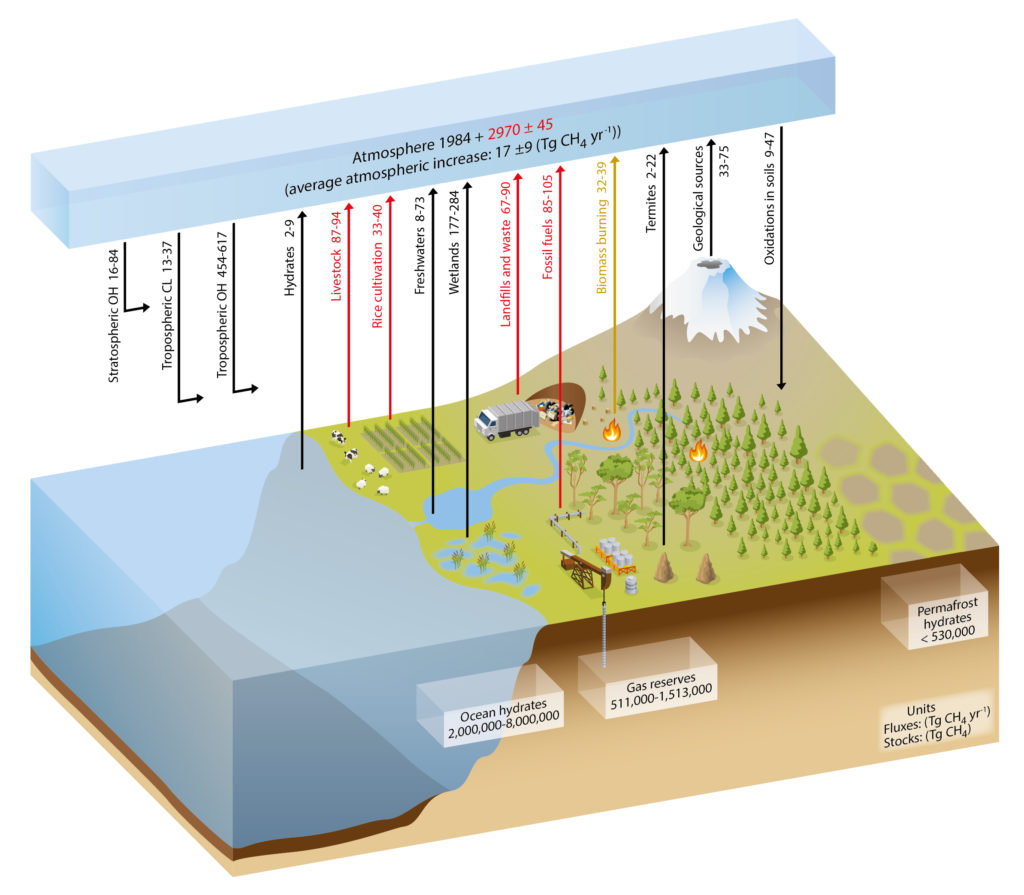
\includegraphics[width=0.9\linewidth]{bilder/IPCC_Cycles_methane.jpg}
				\caption{Vereinfachte Abbildung zum Methankreislauf, Quelle: IPCC 2013, Kapitel 6}
			\end{figure}
		\column{0.35\linewidth}
			Der Gehalt an Methan in der Atmosphäre hat sich zwischen 1750 und 2011 um \SI{250}{\%} erhöht.
	\end{columns}

	\note{
		\begin{itemize}
			\item[] Auch diese Abbildung ist aus dem IPCC Report von 2013
			\item[] schwarze Pfeile stellen wieder vorindustrielle jährliche Flüsse dar
			\item[] rote Pfeile wieder mittlere jährliche Flüsse zwischen 2000 und 2009
			\item[] Die Speicher/Reservoire sind auch wieder als \textbf{Gesamtwert} angegeben
			\item[] vorindustielles Methan in der Atmosphäre: 1984, heutig: +2970 $\rightarrow$ insgesamt also 4954 Tg Methan
			\item[] Methan: järliches atmosphärisches Plus: 17 (+-9) Tg
			\item[] zusätzliches Methan wird freigesetzt durch:
			\begin{itemize}
				\item[] Fossile Brennstoffe: 85-105 Tg
				\item[] Massentierhaltung: 87-94 Tg
				\item[] ganz stark aus Müllhalden (land fills): 67 - 90 Tg
				\item[] $\rightarrow$ durch den anaeroben Abbau der dort gelagerten Stoffe wird von den Mikroorganismen Methan freigesetzt
				\item[] und auch Reisanbau: 33-40 Tg
			\end{itemize}
			\item[] die globalen Speicher von Methan in der Erde sind zusätzlich sehr groß: z.B. Ozean bis zu 8 Mio Tg Methan
		\end{itemize}
	}

\end{frame}

\begin{frame}
	\frametitle{Atmosphärisches Lachgas}
	\begin{columns}
		\column{0.75\linewidth}
			\begin{figure}
				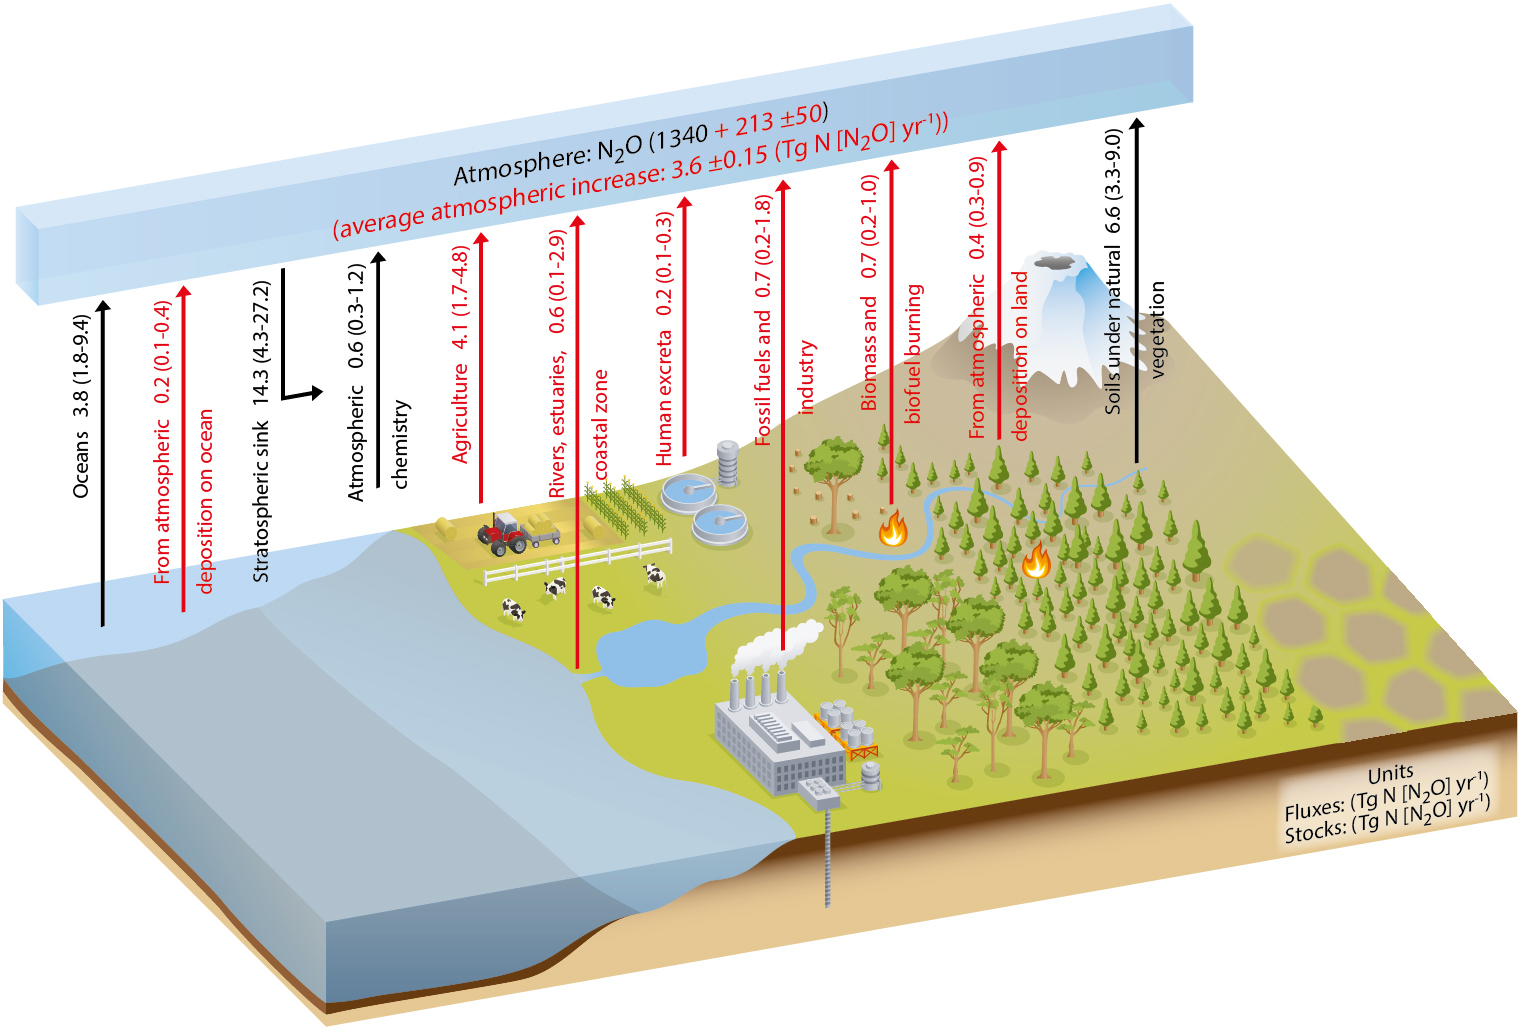
\includegraphics[width=0.9\linewidth]{bilder/IPCC_Cycles_n2o_new.jpg}
				\caption{Vereinfachte Abbildung zum Lachgaskreislauf, Quelle: IPCC 2013, Kapitel 6}
			\end{figure}
		\column{0.25\linewidth}
			Der Gehalt an Lachgas in der Atmosphäre hat sich zwischen 1750 und 2011 um 20 \,\% erhöht.
	\end{columns}

	\note{
		\begin{itemize}
			\item[] Auch diese Abbildung ist aus dem IPCC Report von 2013
			\item[] vorindustielles Lachgas in der Atmosphäre: 1340, heutig: + 213 $\rightarrow$ insgesamt 1553 Tg N$_2$O
			\item[] Lachgas: järliches atmosphärisches Plus: 3,6 (+-0,15) Tg
			\item[] Lachgas v.a. aus Landwirtschaft (4,1 Tg jährliche Emissionen) Verbrennung von Biomasse und Waldrodung

			\item[] \textbf{Fazit:} durch die starke Treibhauswirksamkeit von Methan und Lachgas, sind diese Entwicklung extrem kritisch zu beobachten!
			\item[] Einsparungen in diesem Bereich würden kurzfristig helfen, durch die kürzere Verweildauer, sind sie langfristig aber exakt mit CO$_2$ zu vergleichen
		\end{itemize}
		Fragen? $\rightarrow$ Sonst Restbudget
	}

\end{frame}
